\newcommand{\empt}[2]{$#1^{\langle #2 \rangle}$}

\begin{center}
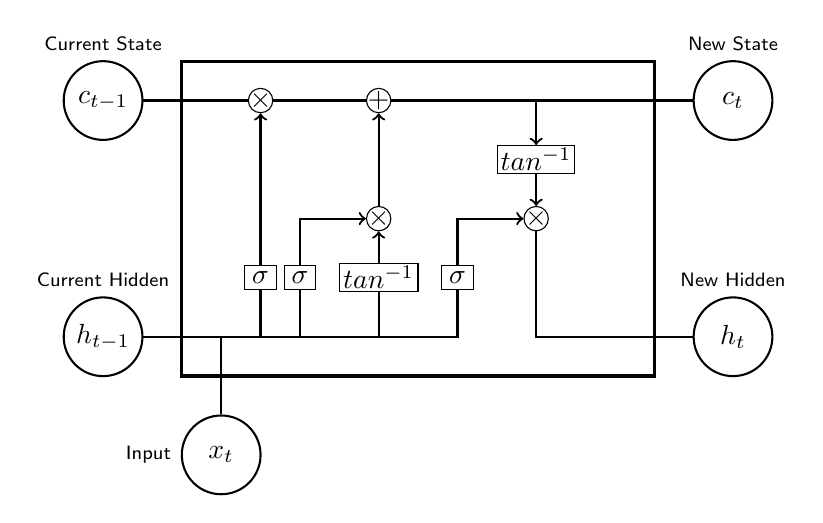
\begin{tikzpicture}[
    cell/.style={
        rectangle, 
        draw,
        very thick,
        },
    operator/.style={
        circle,
        draw,
        inner sep=-0.5pt,
        minimum height =.2cm,
        },
    function/.style={
        ellipse,
        draw,
        inner sep=1pt
        },
    ct/.style={
        circle,
        draw,
        line width = .75pt,
        minimum width=1cm,
        inner sep=1pt,
        },
    gt/.style={
        rectangle,
        draw,
        minimum width=4mm,
        minimum height=3mm,
        inner sep=1pt
        },
    mylabel/.style={
        font=\scriptsize\sffamily
        },
    ArrowC1/.style={
        thick,
        },
    ArrowC2/.style={
        thick,
        },
    ]

    \node [cell, minimum height =4cm, minimum width=6cm] at (0,0){} ;

    \node [gt] (ibox1) at (-2,-0.75) {$\sigma$};
    \node [gt] (ibox2) at (-1.5,-0.75) {$\sigma$};
    \node [gt, minimum width=1cm] (ibox3) at (-0.5,-0.75) {$tan^{-1}$};
    \node [gt] (ibox4) at (0.5,-0.75) {$\sigma$};

    \node [operator] (mux1) at (-2,1.5) {$\times$};
    \node [operator] (add1) at (-0.5,1.5) {+};
    \node [operator] (mux2) at (-0.5,0) {$\times$};
    \node [operator] (mux3) at (1.5,0) {$\times$};
    \node [gt] (func1) at (1.5,0.75) {$tan^{-1}$};

    \node[ct, label={[mylabel]Current State}] (c) at (-4,1.5) {$c_{t-1}$};
    \node[ct, label={[mylabel]Current Hidden}] (h) at (-4,-1.5) {$h_{t-1}$};
    \node[ct, label={[mylabel]left:Input}] (x) at (-2.5,-3) {$x_t$};

    \node[ct, label={[mylabel]New State}] (c2) at (4,1.5) {$c_t$};
    \node[ct, label={[mylabel]New Hidden}] (h2) at (4,-1.5) {$h_t$};
 
    \draw [ArrowC1] (c) -- (mux1) -- (add1) -- (c2);

    \draw [ArrowC2] (h) -| (ibox4);
    \draw [ArrowC1] (h -| ibox1)++(-0.5,0) -| (ibox1); 
    \draw [ArrowC1] (h -| ibox2)++(-0.5,0) -| (ibox2);
    \draw [ArrowC1] (h -| ibox3)++(-0.5,0) -| (ibox3);
    \draw [ArrowC1] (x) -- (x |- h)-| (ibox3);

    \draw [->, ArrowC2] (ibox1) -- (mux1);
    \draw [->, ArrowC2] (ibox2) |- (mux2);
    \draw [->, ArrowC2] (ibox3) -- (mux2);
    \draw [->, ArrowC2] (ibox4) |- (mux3);
    \draw [->, ArrowC2] (mux2) -- (add1);
    \draw [->, ArrowC1] (add1 -| func1)++(-0.5,0) -| (func1);
    \draw [->, ArrowC2] (func1) -- (mux3);

    \draw [-, ArrowC2] (mux3) |- (h2);

\end{tikzpicture}
\end{center}